\section{Simulation Procedure} \label{sec:sim_procedure}

Now that a flight certification maneuver has been chosen, a method to run a current aircraft design thorough the maneuver-of-interest needs to be be developed.
The aircraft design is represented using probabilistic multi-fidelity aerodynamics and controls databases as shown in \ref{sec:gtt_dbs}.
The uncertainty in the data that informs the databases, manifests itself in slight variations in the samples of the databases.
Each sample aerodynamic database has information about the forces and moments on an aircraft at various points in the flight envelope.
The controls database samples contain information about the moments induced on the aircraft due to various control surface deflections. 
These samples are run through flight simulation software that can integrate the force and moment information, combine it with the effects of control inputs, and perform a time-accurate maneuver that is defined in the simulation software. 

This part of the work leans heavily on the expertise of the The Boeing Company in flight simulation and control law mixing.
Due to proprietary and patent restrictions, exact implementation of the flight simulation code is unavailable but enough information is provided to outline the simulations' overarching methodology and workflow.

Instead of a full 6 Degree of Freedom (DoF) flight simulation, a slightly simplified 5 DoF flight simulation tool, ignoring displacements in y-axis (body fitted coordinate system), is used.
While this is slightly less accurate than a 6DoF simulation, it is well suited for Monte Carlo analysis which requires the rapid analysis of hundreds of aircraft databases.
Another simplification is that the maneuver is not performed in a closed-loop, trajectory-following manner. 
Instead, the maneuver is first processed into a set of rotational accelerations that are required to complete the maneuver, and then the control inputs needed to provide those accelerations are calculated. 
If the aircraft is able to perform the maneuver without over-saturating any of the control surface deflections, the maneuver is considered a success.

For this section, the results use the single-fidelity aerodynamics and controls databases that are created using experimental data from the NAART and FVWT experimental campaigns (Section \ref{sec:gtt_dbs}). 
Multi-fidelity databases are used and compared for the results in Section \ref{sec:cba_results}.

\subsection{Maneuver Simulation}

Figure \ref{fig:cfr147d_inputs} represents the steps required to simulate the airworthiness test. 
The first step is to convert the maneuver of interest, in this case the \textit{Lateral Control: Roll Capability \S 25.147(d)} maneuver, into an appropriate trajectory for the aircraft to follow. 
The trajectory is defined as a time history of the aircraft's orientation that would be required to meet the parameters of the maneuver. 
This particular maneuver is mostly defined by the roll angle of the aircraft and is shown as a function of time in Figure \ref{subfig:roll_angle}.
There are other parameters included in the trajectory definition, for example the pitch angle required to maintain constant altitude, but the roll angle defines the trajectory of the certification maneuver, and is the focus here.
The aircraft starts with steady level flight, rolls to an angle $\psi = +30^\circ$, and then completes the roll maneuver from $\psi = +30^\circ$ to $=-30^\circ$ in 11 seconds, as required by the certification maneuver. 

The second step of the simulation process is to use the geometric properties and the aerodynamics database of the aircraft to calculate the accelerations that would be required to follow the trajectory.
This involves time-stepping through the trajectory definition and calculating the directional and rotational accelerations that would put the aircraft in the appropriate orientation at the next time step. 
Figure \ref{subfig:roll_acc} shows the roll acceleration vs. time that would be required to execute the maneuver.
There are a few distinct sections of the roll acceleration plot. 
For the first second, to establish steady trimmed flight, the aircraft stays level and the roll acceleration stays at zero.
A large positive acceleration is required to start the roll to a bank angle of $+30^\circ$. 
It tapers off to nearly zero at $13$ seconds, after which a moderate negative roll acceleration is required to stabilize the aircraft at that bank angle. 
The heart of the certification maneuver starts at $16$ seconds, as indicated by the negative peak for the roll acceleration.
The required acceleration reduces as the bank angle approaches zero, and then peaks again, once it is past $\psi=0^\circ$.
Finally, around the $27$ second mark, a sharp positive roll acceleration is required to stabilize the aircraft at the $-30^\circ$ bank angle. 
The acceleration definitions from this step are fed into the next step.

The final step in the simulation procedure involves using the controls database of the aircraft, and The Boeing Company's patented control law mixer \cite{control_law_patent}, to compute the control surface deflections needed to provide the accelerations that the maneuver demands.
This is done by time-stepping through the acceleration definitions from the previous simulation step, and calculating the control inputs that would be required to meet the acceleration demands at that time step. 
The right and left aileron deflections required to achieve the roll accelerations defined in Figure \ref{subfig:roll_acc}, are shown in Figure \ref{subfig:ail_defl}.
The mostly linear relationship between aileron deflection and the resulting roll acceleration leads to the control surface deflections mimicking the trends seen in the roll acceleration plot. 

\begin{figure}
    \centering
    \begin{subfigure}[Flight simulation trajectory definition for the roll angle of the aircraft. Derived from the air-worthiness test.] {
        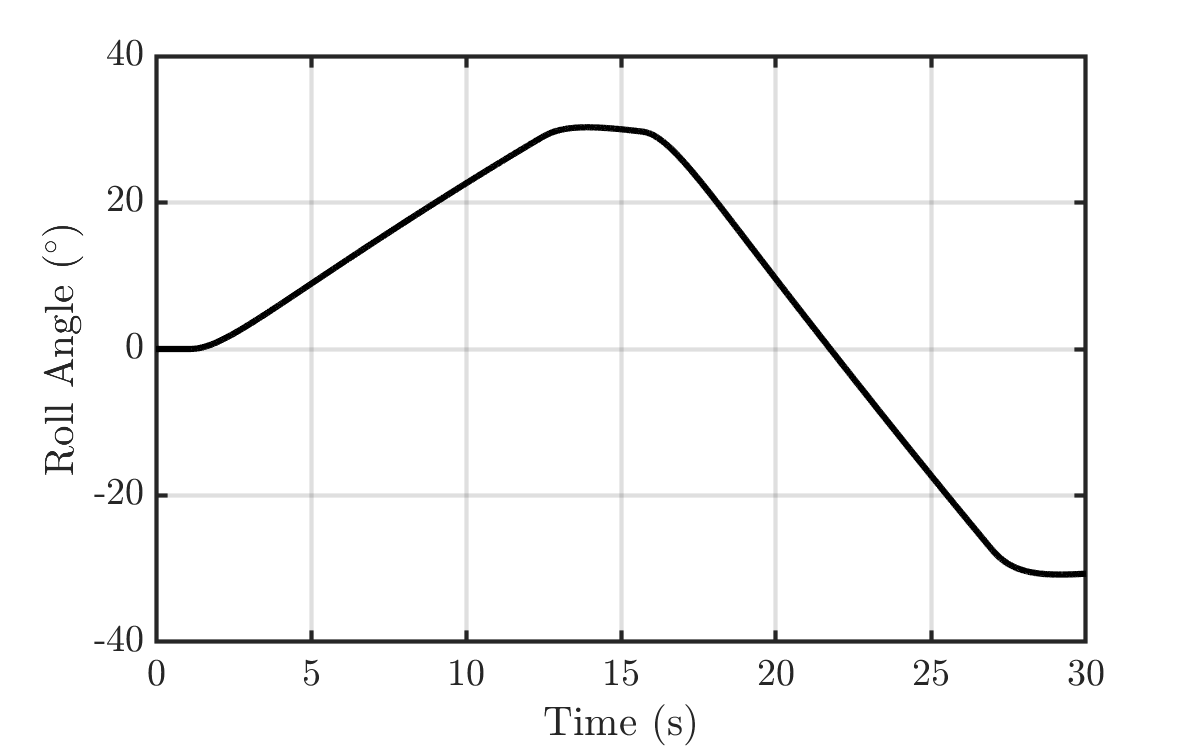
\includegraphics[trim=0 0 0 0, clip, width=.55\textwidth]{code/image_gen/cba/images/cfr147d_roll_angle.png}
        \label{subfig:roll_angle}
    }
    \end{subfigure}
    \hfill
    \begin{subfigure}[Roll acceleration that would be required for the aircraft to follow the roll angle trajectory]{
        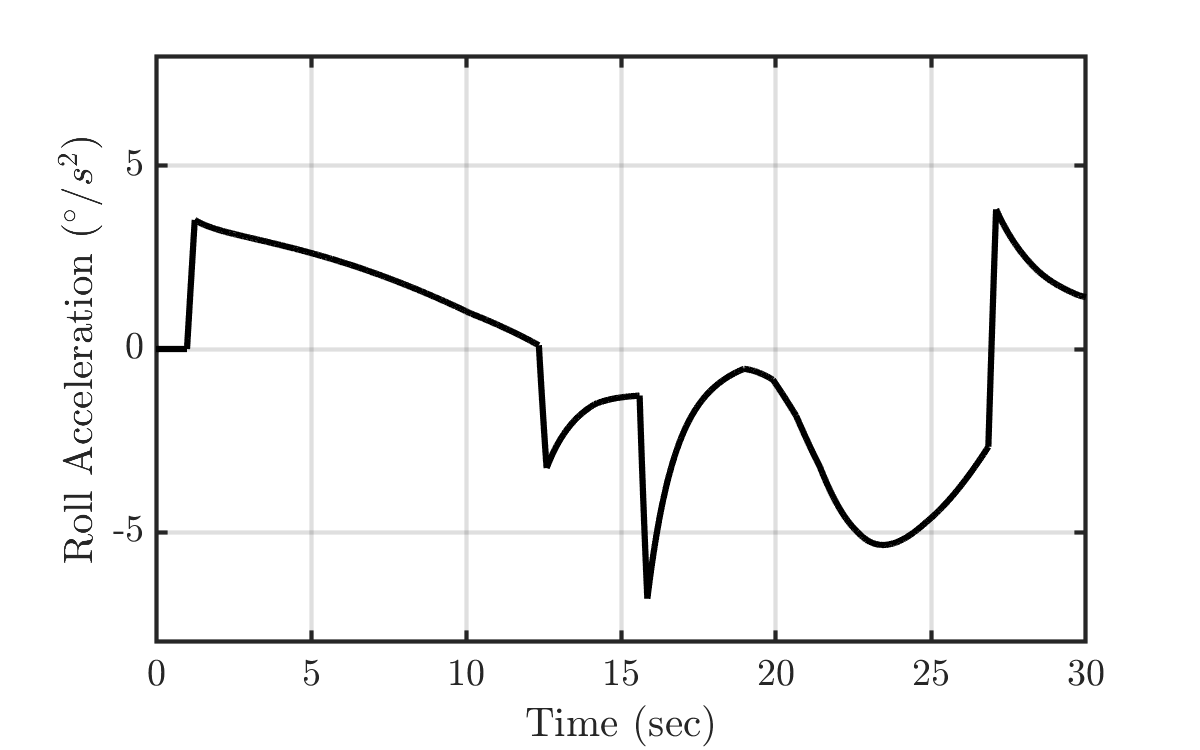
\includegraphics[trim=0 0 0 0, clip, width=.55\textwidth]{code/image_gen/cba/images/cfr147d_roll_acc.png} 
        \label{subfig:roll_acc}
    } 
    \end{subfigure}
    \hfill
    \begin{subfigure}[Left and right aileron deflections commanded to create the requisite roll accelerations]{
        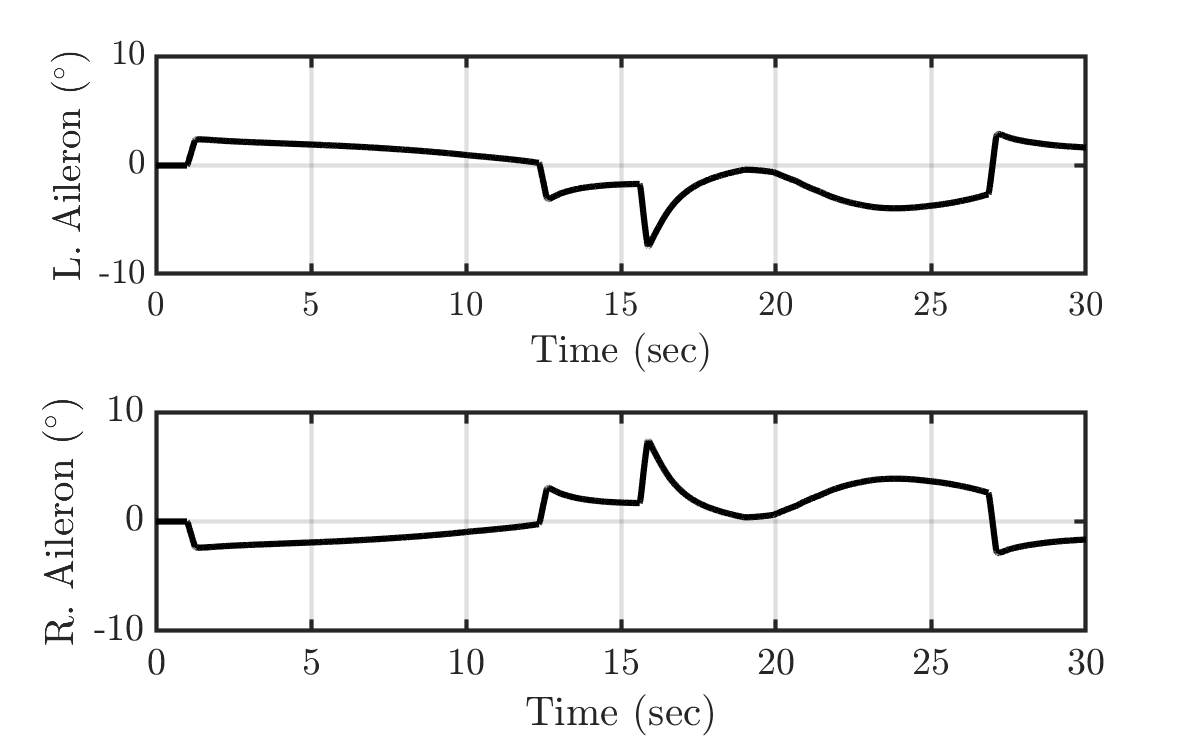
\includegraphics[trim=0 0 0 0, clip, width=.55\textwidth]{code/image_gen/cba/images/cfr147d_ail_defl.png} 
        \label{subfig:ail_defl}
    } 
    \end{subfigure}
    \caption{Steps required to convert the air-worthiness test into a the required inputs for the flight simulation of the maneuver. \label{fig:cfr147d_inputs}}
\end{figure}

Other parameters in the trajectory definition, such as minimizing sideslip or maintaining altitude, necessitate yaw and pitch accelerations.
These are shown in Figure \ref{subfig:yaw_acc} and \ref{subfig:pitch_acc}.
In turn, these require rudder and elevator inputs that are shown in Figure \ref{subfig:rud_defl} and \ref{subfig:elev_defl}. 
Again, the linear relationship between the rotational accelerations, yawing and pitching moments, and the corresponding control surface deflections, rudder and elevator, results in the acceleration trends being closely matched by the surface deflection trends. 
As long as the surface deflections that are commanded by the flight simulator don't exceed the physical limit of the available control surface deflection, the maneuver can be completed and is considerd a success. 

\begin{figure}
    \centering
    \begin{subfigure}[Yaw acceleration required during the maneuver to minimize sideslip.] {
        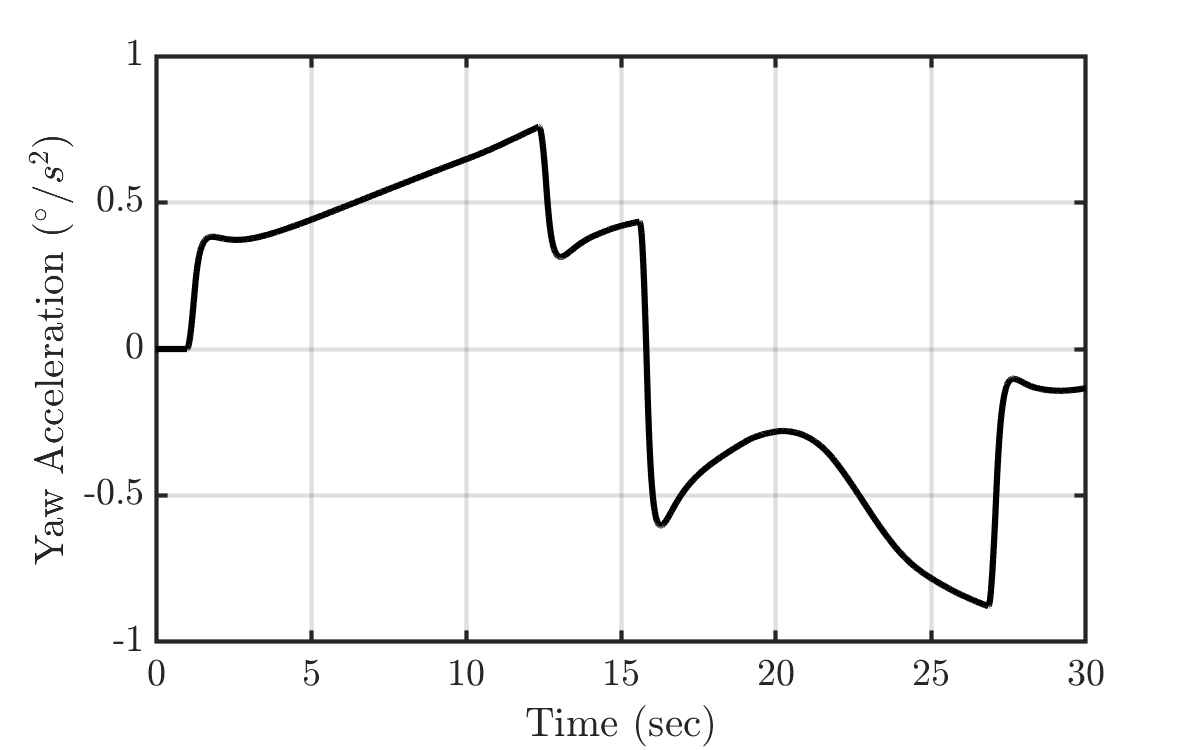
\includegraphics[trim=0 0 0 0, clip, width=.48\textwidth]{code/image_gen/cba/images/cfr147d_yaw_acc.png}
        \label{subfig:yaw_acc}
    }
    \end{subfigure}
     \hfill
    \begin{subfigure}[Pitch acceleration required during the maneuver to maintain altitude.]{
        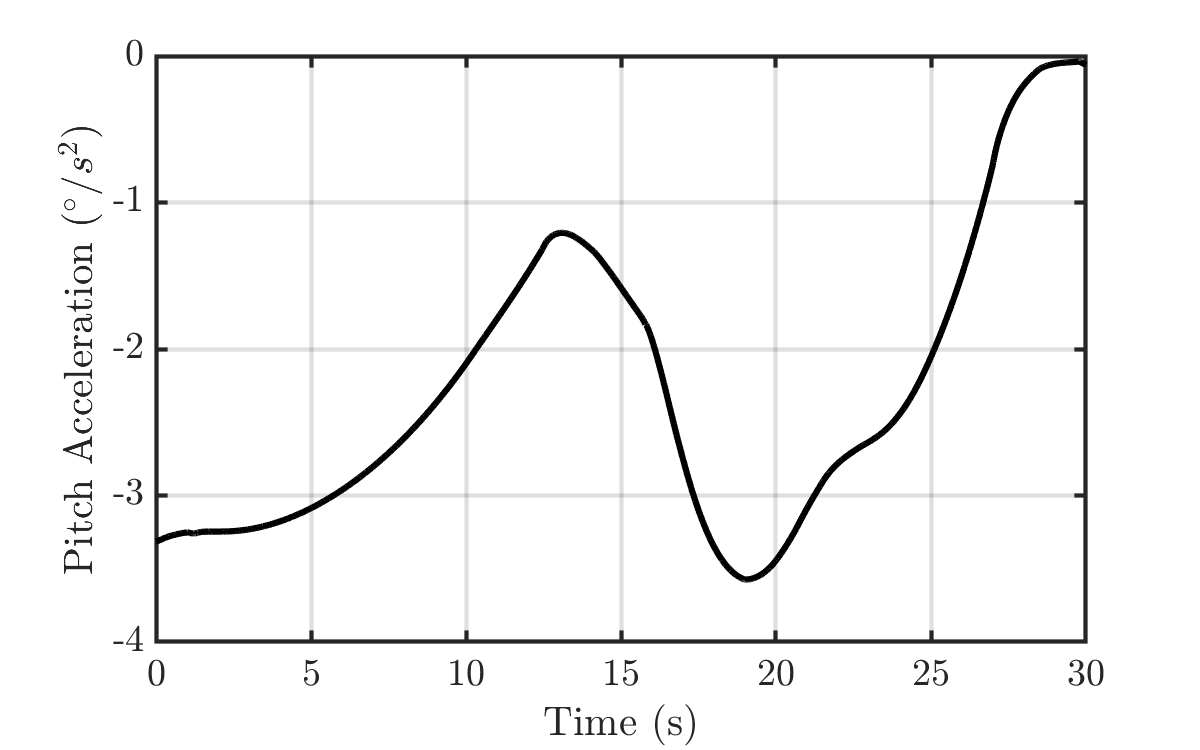
\includegraphics[trim=0 0 0 0, clip, width=.48\textwidth]{code/image_gen/cba/images/cfr147d_pitch_acc.png} 
        \label{subfig:pitch_acc}
    } 
    \end{subfigure}
    \hfill
    \begin{subfigure}[Rudder deflection required to minimize sideslip.]{
        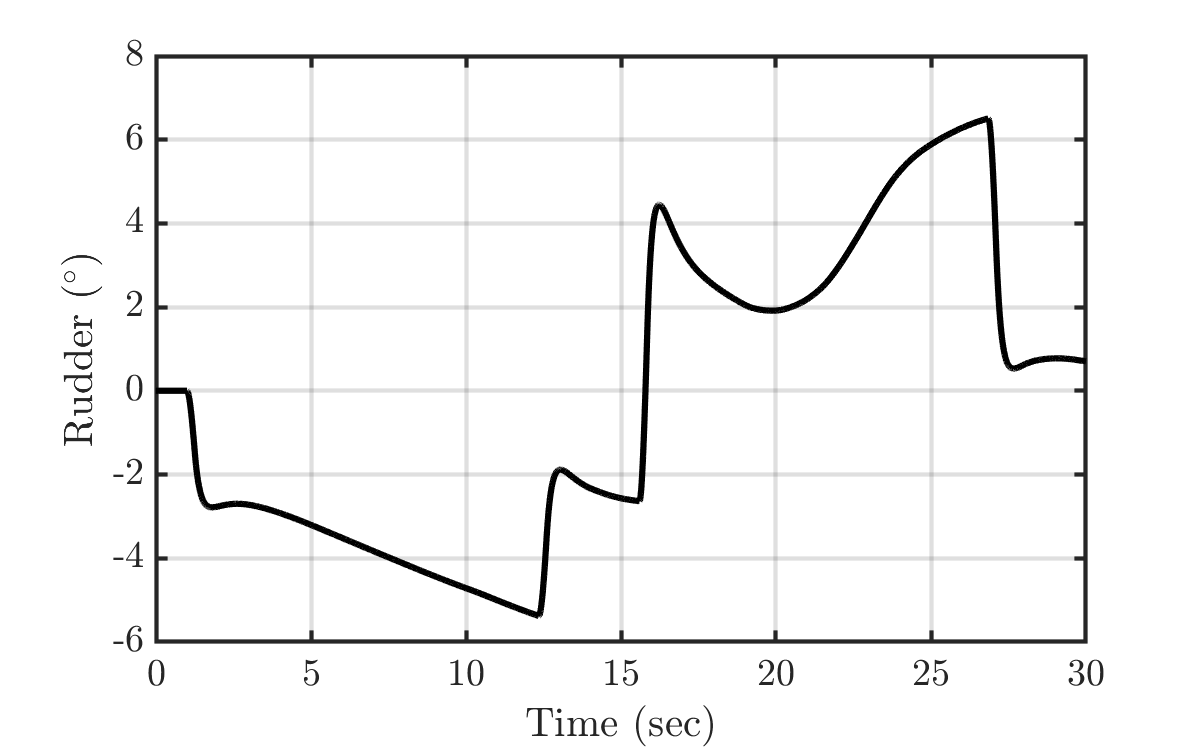
\includegraphics[trim=0 0 0 0, clip, width=.48\textwidth]{code/image_gen/cba/images/cfr147d_rud_defl.png} 
        \label{subfig:rud_defl}
    } 
    \end{subfigure}
    \hfill
    \begin{subfigure}[Elevator deflection required to maintain altitude during the banked turn.]{
        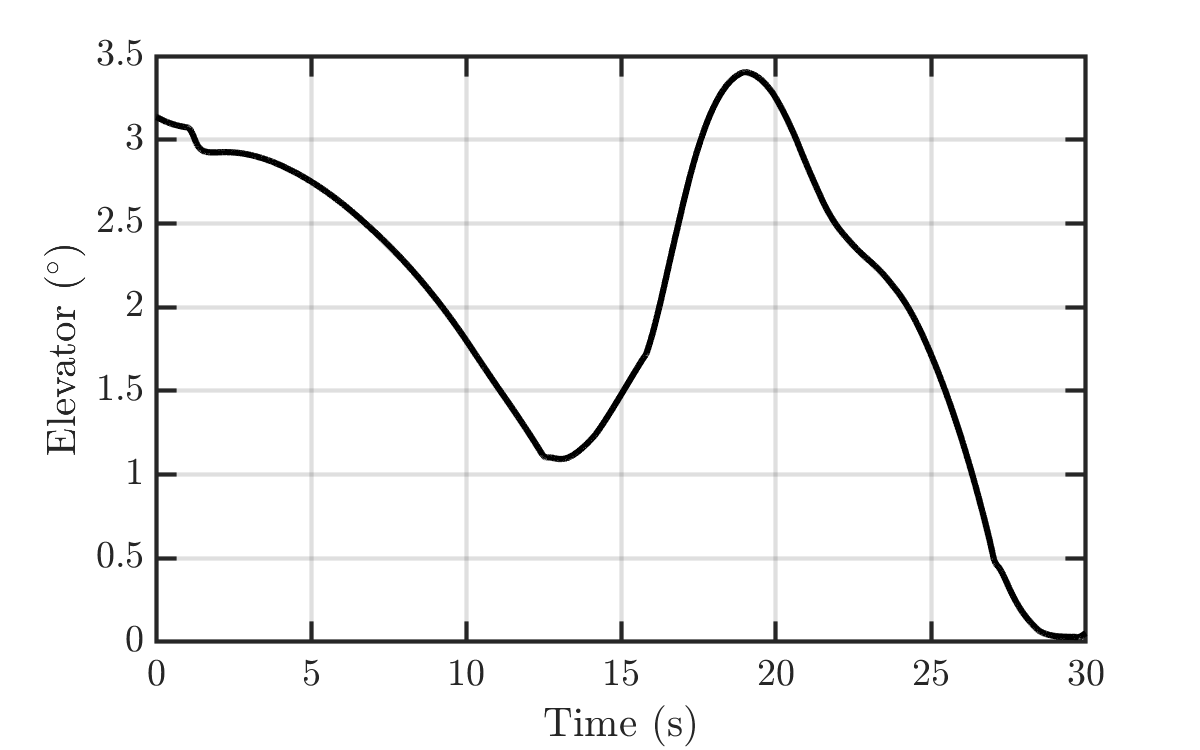
\includegraphics[trim=0 0 0 0, clip, width=.48\textwidth]{code/image_gen/cba/images/cfr147d_elev_defl.png} 
        \label{subfig:elev_defl}
    } 
    \end{subfigure}
    \caption{Rudder and elevator control inputs are required to satisfy the yaw and pitch accelerations needed to complete the maneuver.  \label{fig:cfr147d_pitch_yaw_inputs}}
\end{figure}

\subsection{Engine Failure Simulations}
As stated in Section \ref{sec:maneuver}, the certification maneuver needs to completed with one engine inoperative.
Specifically, the inoperative engine should be the one that makes the maneuver more difficult.
In the coordinate system defined by the $x$-axis pointing out of the nose and the $z$-axis pointing down towards the ground, the roll from $\psi = +30^\circ$ to $\psi = -30^\circ$ is made more difficult with the right engine inoperative. 
The asymmetric thrust causes the aircraft to yaw towards the inoperative engine, creating a rolling moment in the direction opposite to the roll maneuver.

This can be confirmed by looking at Figure \ref{fig:eo_cfr147d_inputs}. 
There are three configurations for which the time history of the rotational accelerations (left column) and the control surface deflections (right column) are plotted.
The blue line represents the nominal configuration with both engines operating. 
The red line represents the case with an inoperative right engine (Right Engine Out) and the yellow line represents the case with an inoperative left engine (Left Engine Out).
Since the engines are aligned with the $x$-axis, the asymmetric thrust does not induce any rolling moment and Figure \ref{subfig:eo_roll_acc} shows identical roll acceleration requirements for all three configurations.
However, it does induce yawing and pitching moments. 
The direction of the yawing moment depends on which engine is inoperative.
Consequently, Figure \ref{subfig:eo_yaw_acc} shows the required yaw accelerations for the engine out cases to be symmetric about the nominal condition. 
The induced pitching moment is independent of which engine is inoperative, and Figure \ref{subfig:eo_pitch_acc} confirms this with the red and yellow lines being coincident. 

Even though the roll acceleration requirements are identical, the roll-yaw coupling necessitates different aileron deflections for the different configurations, as seen in Figure \ref{subfig:eo_ail_defl}. 
Similar trends are seen for the rudder and elevator deflections in Figures \ref{subfig:eo_rud_defl} and \ref{subfig:eo_elev_defl} respectively. 
The configuration that makes the maneuver more difficult would be the one that requires higher control surface deflection angles. 
These figures show that the right engine out case (red line) requires higher aileron deflections, similar rudder deflections, and slightly higher elevator deflections. 
This confirms that having an inoperative engine on the right side of the aircraft makes the maneuver more difficult.

\begin{figure}
    \centering
    \begin{subfigure}[Roll accelerations vs. time.] {
        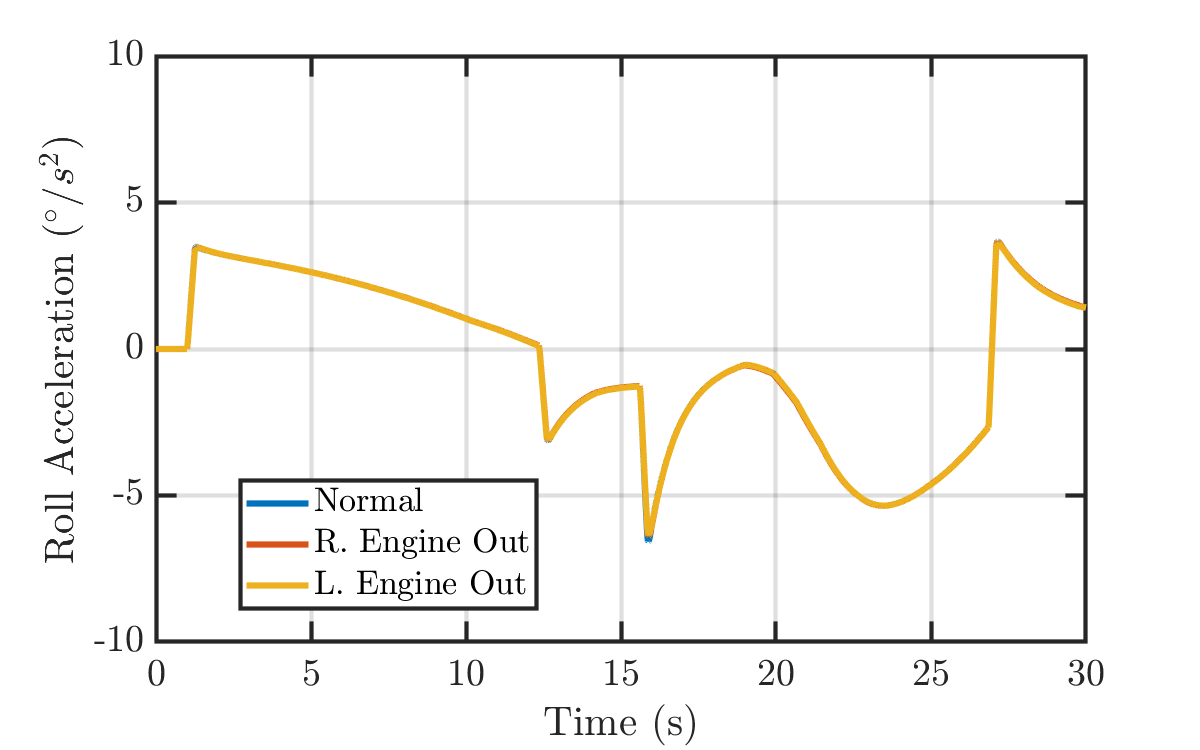
\includegraphics[trim=0 0 0 0, clip, width=.48\textwidth]{code/image_gen/cba/images/eo_cfr147d_roll_acc.png}
        \label{subfig:eo_roll_acc}
    }
    \end{subfigure}
     \hfill
     \begin{subfigure}[Aileron deflections vs. time.]{
        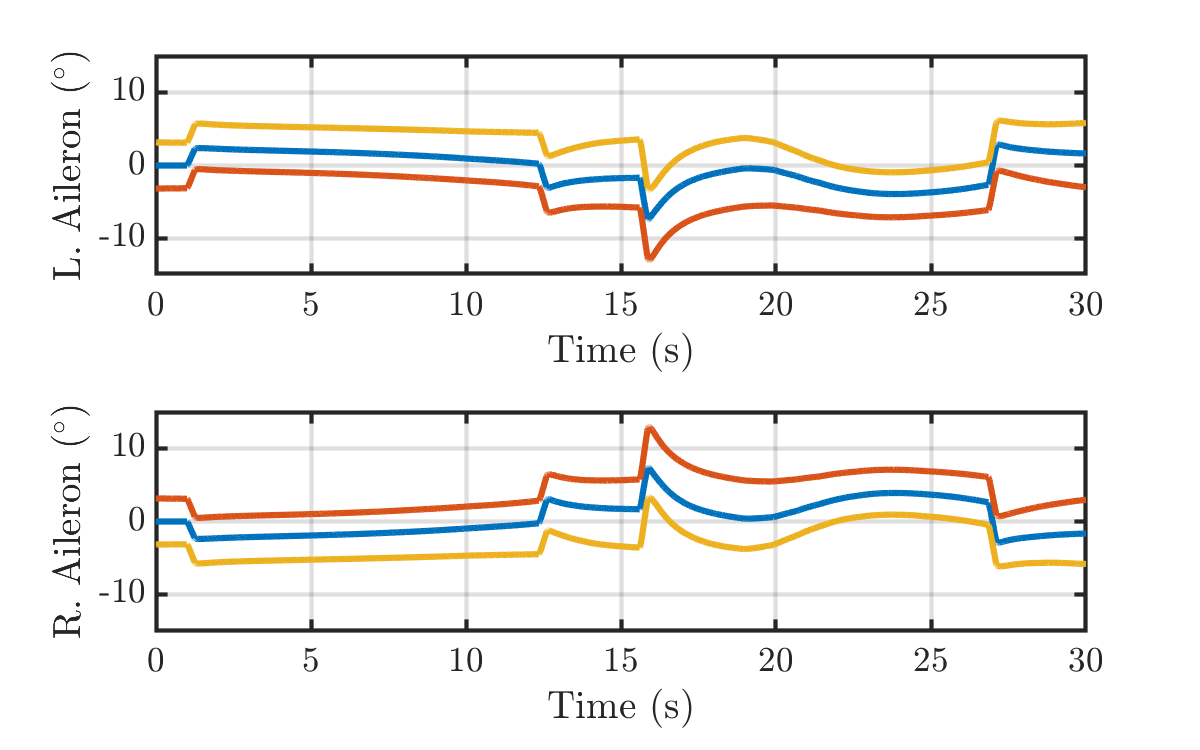
\includegraphics[trim=0 0 0 0, clip, width=.48\textwidth]{code/image_gen/cba/images/eo_cfr147d_ail_defl.png} 
        \label{subfig:eo_ail_defl}
    } 
    \end{subfigure}
    \hfill
    \begin{subfigure}[Yaw accelerations vs. time.] {
        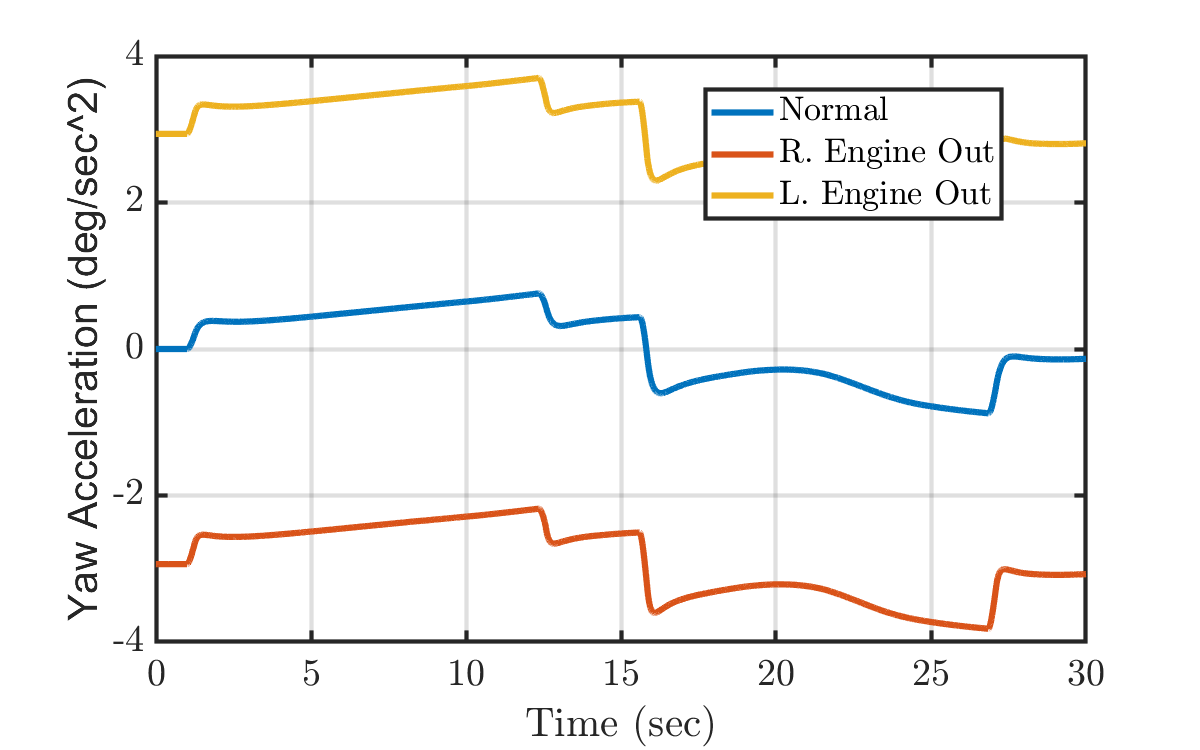
\includegraphics[trim=0 0 0 0, clip, width=.48\textwidth]{code/image_gen/cba/images/eo_cfr147d_yaw_acc.png}
        \label{subfig:eo_yaw_acc}
    }
    \end{subfigure}
    \hfill
    \begin{subfigure}[Rudder deflections vs. time.]{
        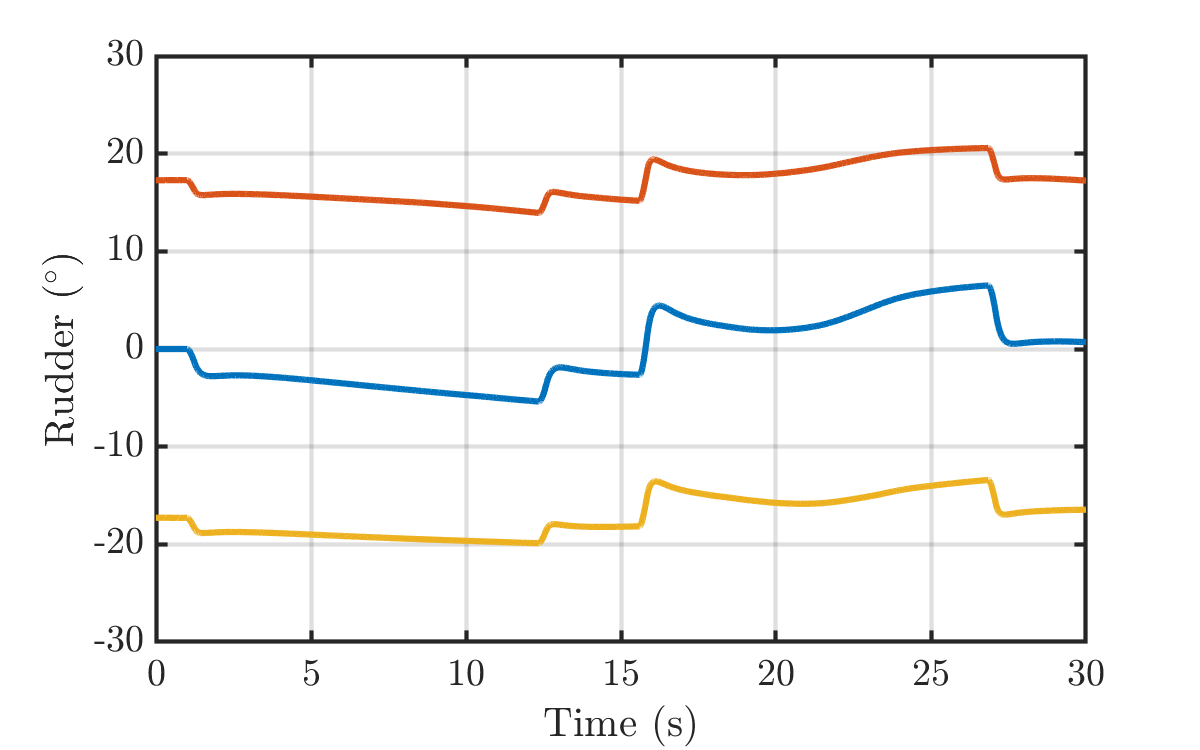
\includegraphics[trim=0 0 0 0, clip, width=.48\textwidth]{code/image_gen/cba/images/eo_cfr147d_rud_defl.png} 
        \label{subfig:eo_rud_defl}
    } 
    \end{subfigure}
     \hfill
    \begin{subfigure}[Pitch accelerations vs. time.]{
        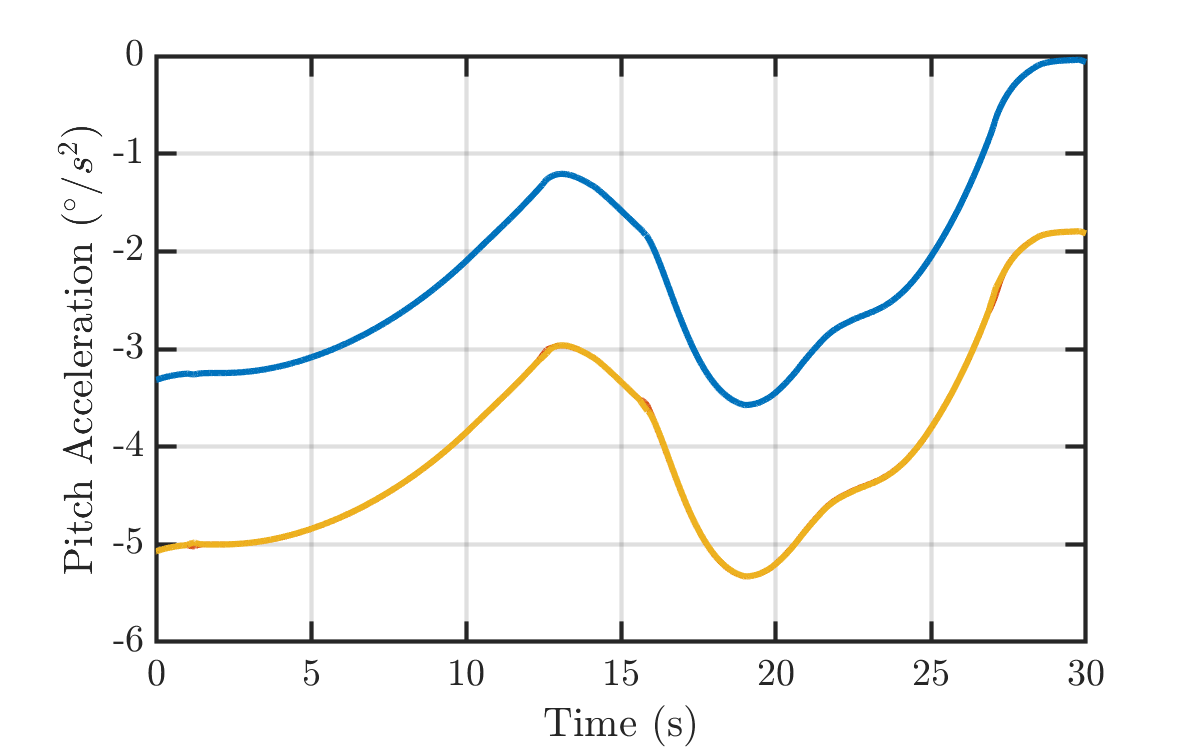
\includegraphics[trim=0 0 0 0, clip, width=.48\textwidth]{code/image_gen/cba/images/eo_cfr147d_pitch_acc.png} 
        \label{subfig:eo_pitch_acc}
    } 
    \end{subfigure}
    \hfill
    \begin{subfigure}[Elevator deflections vs. time.]{
        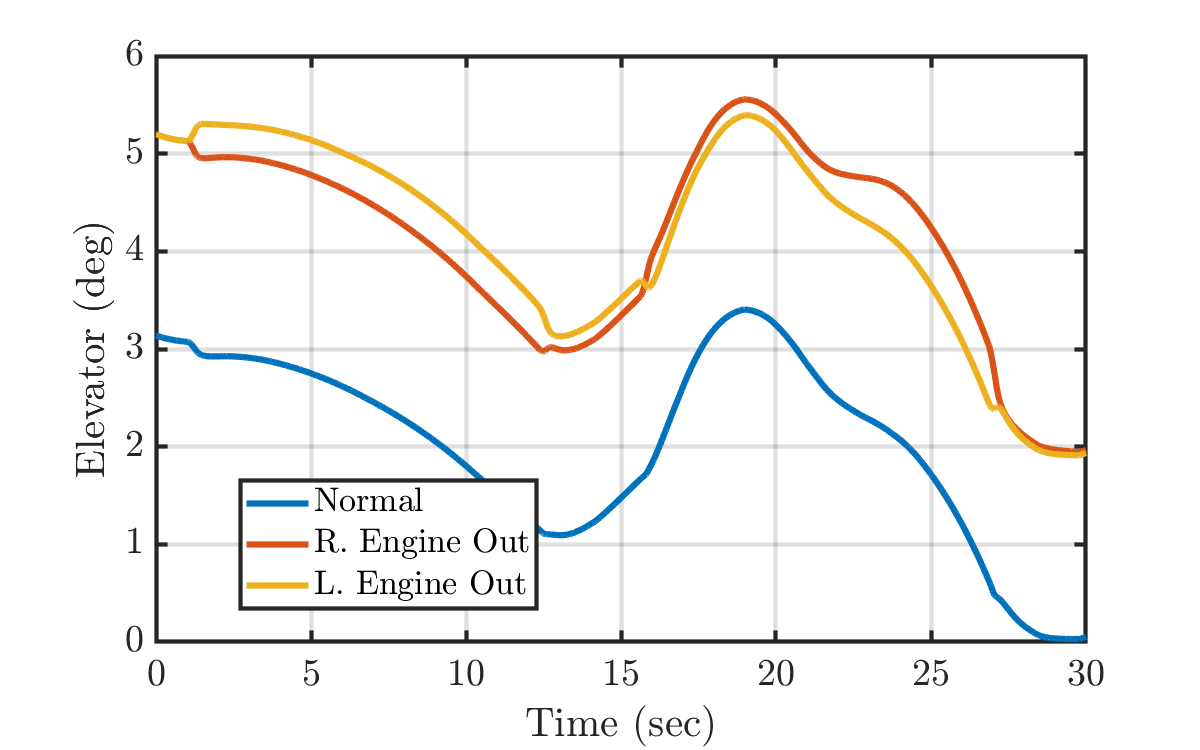
\includegraphics[trim=0 0 0 0, clip, width=.48\textwidth]{code/image_gen/cba/images/eo_cfr147d_elev_defl.png} 
        \label{subfig:eo_elev_defl}
    } 
    \end{subfigure}
    \caption{Rotational accelerations and control surface deflections required to perform the maneuver with both engines operative (blue), right engine inoperative (red), and left engine inoperative (yellow). \label{fig:eo_cfr147d_inputs}}
\end{figure}

% \subsection{Maneuver Simulation}
% Armed with the aircraft databases and the time history of the necessary control surface deflections,the flight certification maneuver can be flown using Boeing's 5DoF flight simulator. 
% At every time step during the simulation, the aircraft's state, as defined by its orientation and configuration, are tracked.
% The orientation is defined by the angle of attack and angle of sideslip of the aircraft.  
% Configuration refers to aircraft's parameters such as engine thrust, airspeed, flap position etc. 
% The aircraft's aerodynamics database defines the forces and moments that are experienced by the aircraft at that orientation and configuration. 
% The time history of the control surface deflections are translated into their resulting moments using the aircraft's controls database. 
% These forces and moments are integrated in time to calculate the aircraft's orientation and configuration at the next time step. 
% This integration in time is continued until the maneuver is complete.

% The results of one such simulation, with the right engine inoperative, can be seen in Figure \ref{fig:reo_cfr147d_sim}.
% The solid black line represents the preprocessed inputs to the simulator and the red dashed line represents a simulated maneuver.
% The simulation is able to track the trajectory and the roll accelerations exactly as shown by the coincident lines in Figures \ref{subfig:reo_roll_angle} and \ref{subfig:reo_roll_acc}. 
% Figure \ref{subfig:reo_ail_defl} shows the slight changes to the aileron deflection angles in the simulations that ensure the roll acceleration is tracked correctly.

% \begin{figure}
%     \centering
%     \begin{subfigure}[Flight simulation trajectory definition for the roll angle of the aircraft. Derived from the air-worthiness test.] {
%         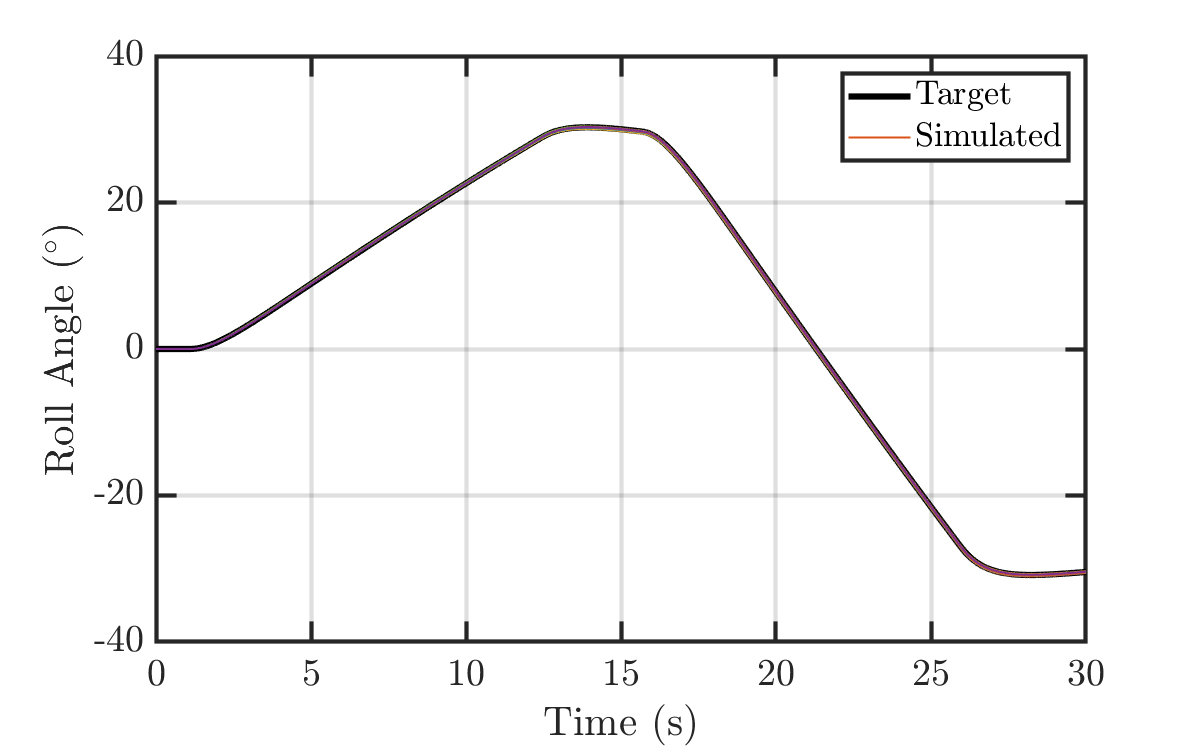
\includegraphics[trim=0 0 0 0, clip, width=.55\textwidth]{code/image_gen/cba/images/reo_cfr147d_roll_angle_mean.png}
%         \label{subfig:reo_roll_angle}
%     }
%     \end{subfigure}
%     \hfill
%     \begin{subfigure}[Roll acceleration that would be required for the aircraft to follow the roll angle trajectory]{
%         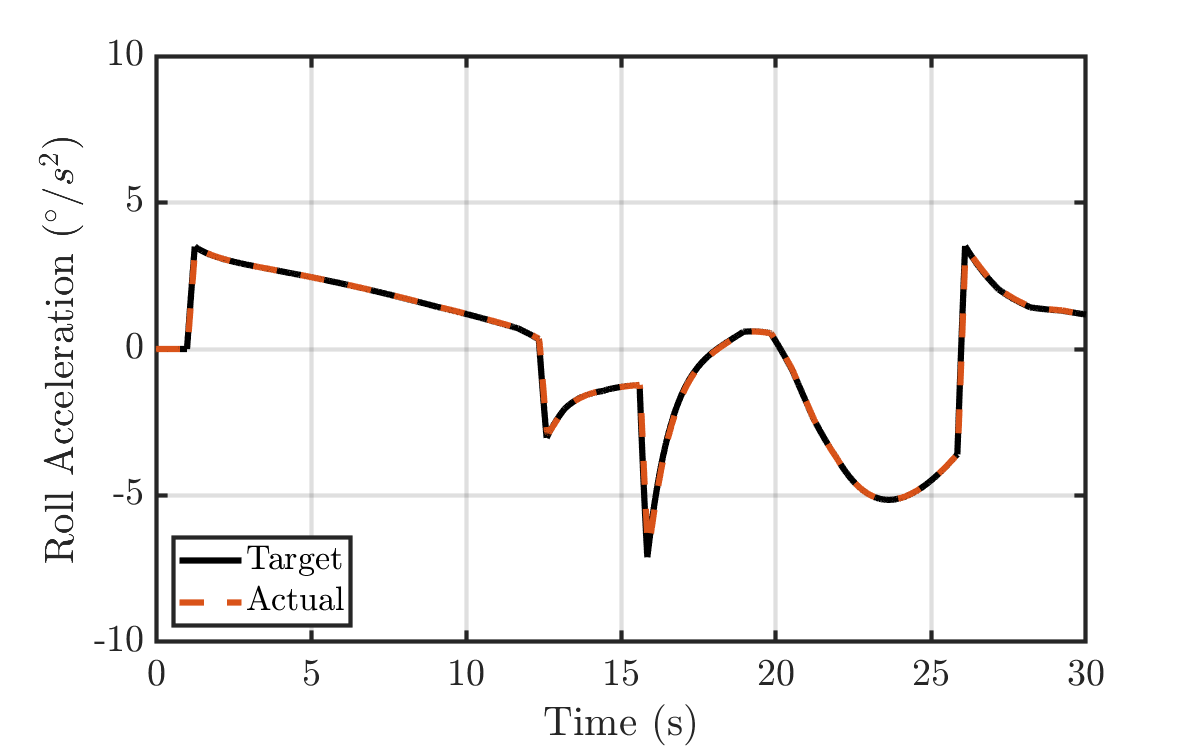
\includegraphics[trim=0 0 0 0, clip, width=.55\textwidth]{code/image_gen/cba/images/reo_cfr147d_roll_acc_mean.png} 
%         \label{subfig:reo_roll_acc}
%     } 
%     \end{subfigure}
%     \hfill
%     \begin{subfigure}[Left and right aileron deflections commanded to create the requisite roll accelerations]{
%         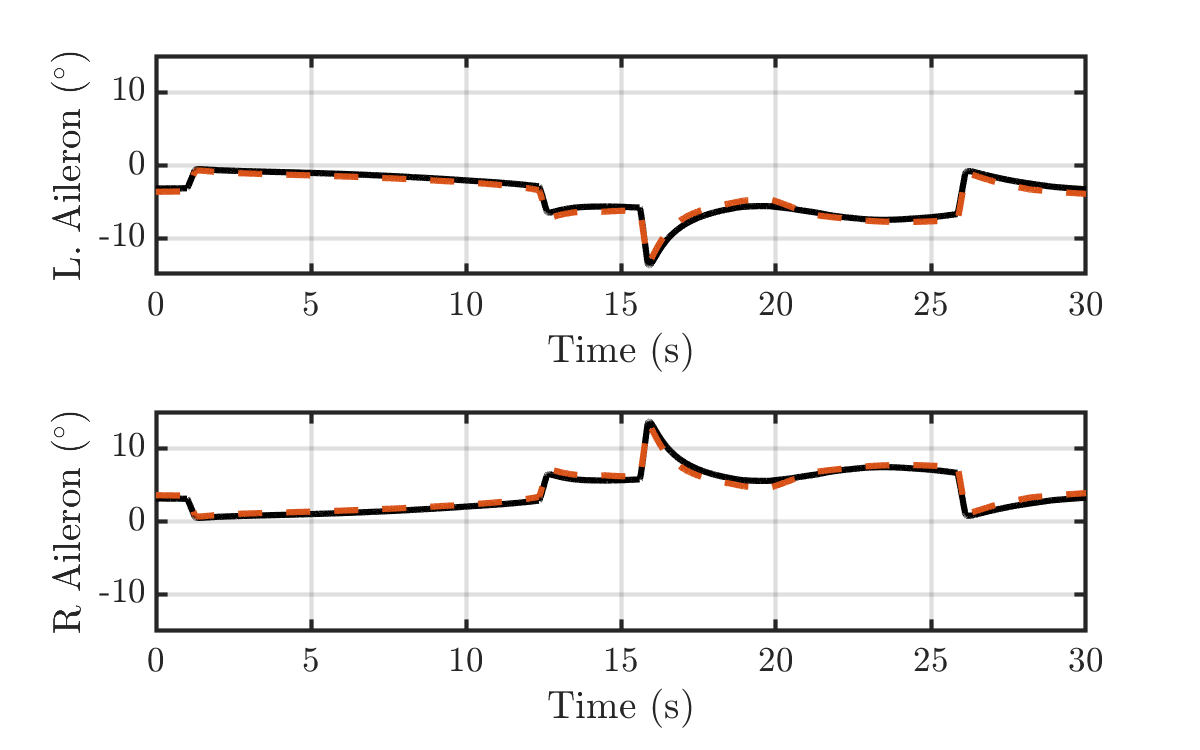
\includegraphics[trim=0 0 0 0, clip, width=.55\textwidth]{code/image_gen/cba/images/reo_cfr147d_ail_defl_mean.png} 
%         \label{subfig:reo_ail_defl}
%     } 
%     \end{subfigure}
%     \caption{Steps required to convert the air-worthiness test into a the required inputs for the flight simulation of the maneuver. \label{fig:reo_cfr147d_sim}}
% \end{figure}

\subsection{Evaluating Success or Failure}

The metric for the successful completion of the certification maneuver is defined in the FAA's guide \cite{romanowski_flight_2018} as being able to perform the $60^\circ$ change in bank angle under 11 seconds. 
Enforcing this criteria directly would require a closed-loop, trajectory-following flight simulation where the aircraft continuously calculates and adjusts the control input required to complete the maneuver as fast as possible without exceeding the physical limits on the control systems. 
In the flight simulation procedure that is used, the time taken to complete the maneuver is predefined.
There is very little variation in actual time taken for the aircraft to complete the maneuver because the control inputs are specifically calculated to complete the maneuver in the predefined time.

To work around this, the metric for success is re-framed. 
Since the time to complete the maneuver is predefined, the metric of success becomes the level of saturation of the control surfaces required to complete the maneuver. 
Specifically, three metrics are defined, one for each rotational acceleration: pitch, roll, yaw. 
These are calculated for a simulated maneuver as
\begin{align}
    \rho_{pitch} = 1- \max\left \{ \frac{\left \vert \delta_e^{req}(t) \right \vert }{\delta_e^{lim}} \right \}
    \\
    \rho_{roll} = 1- \max\left \{ \frac{\left \vert \delta_a^{req}(t) \right \vert }{\delta_a^{lim}} \right \}
    \\
    \rho_{yaw} = 1- \max\left \{ \frac{\left \vert \delta_r^{req}(t) \right \vert }{\delta_r^{lim}} \right \}
\end{align}
where $\delta_e$, $\delta_a$, and $\delta_r$ correspond to elevator, aileron, and rudder deflection angles, respectively.
The superscript $req$ indicates the value that is calculated by the simulator, and the superscript $lim$ indicates the maximum allowable control surface deflection angle. 
The maximum saturation over the entire duration of the flight simulation is taken and subtracted from $1$.
If at any point during the flight simulation a control surface is completely saturated, say $\delta_e^{req} = \delta_e^{lim}$, the corresponding metric is $0$, in this case $\rho_{pitch} = 0$.
The deflection limits for each of the control surfaces is shown in Table \ref{tab:gtt_defl_limits}.

\begin{table}
\centering
    \renewcommand{\arraystretch}{1.2}
    \captionsetup{justification=centering}
    \caption{Control surface deflection limits on the GTT aircraft.} 
    \begin{tabular}{|c|c|}
    \hline
        Control Surface & Deflection limits \\ \hline
        Ailerons & $\pm 25^\circ$ \\ \hline
        Elevator & $\pm 20^\circ$ \\ \hline
        Rudder & $\pm 30^\circ$ \\ \hline
        Spoilers & $\pm 60^\circ$ \\ \hline
        Flaps & $\pm 45^\circ$ \\ \hline
    \end{tabular}
    \label{tab:gtt_defl_limits}
\end{table}

To show a concrete example, the maneuver definition is tweaked to force the over-saturation of the ailerons.
The maneuver is made more aggressive by shortening the time taken to perform the $60^\circ$ change in bank angle from $11 sec$ to $2.5 sec$.
The maneuver trajectory, required roll accelerations, and simulated control surface deflections are shown in 

\begin{figure}
    \centering
    \begin{subfigure}[Flight simulation trajectory definition for the roll angle of the aircraft. Derived from the air-worthiness test.] {
        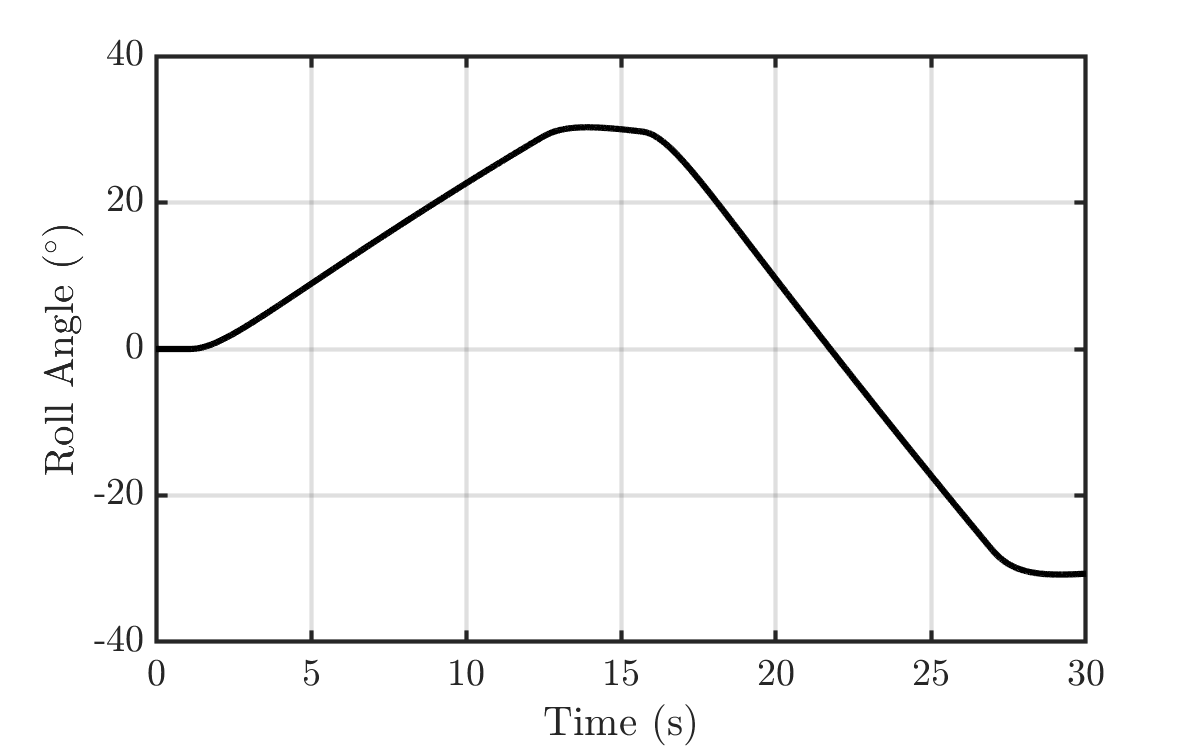
\includegraphics[trim=0 0 0 0, clip, width=.55\textwidth]{code/image_gen/cba/images/cfr147d_roll_angle.png}
        \label{subfig:roll_angle}
    }
    \end{subfigure}
    \hfill
    \begin{subfigure}[Roll acceleration that would be required for the aircraft to follow the roll angle trajectory]{
        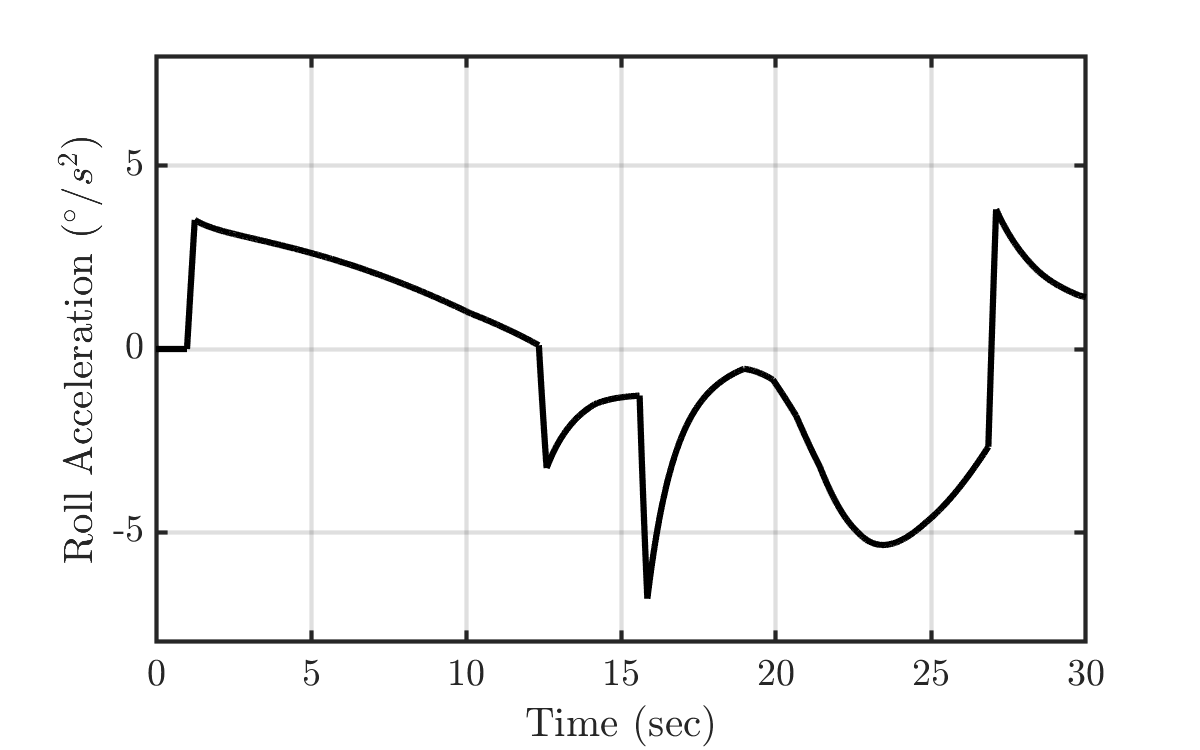
\includegraphics[trim=0 0 0 0, clip, width=.55\textwidth]{code/image_gen/cba/images/cfr147d_roll_acc.png} 
        \label{subfig:roll_acc}
    } 
    \end{subfigure}
    \hfill
    \begin{subfigure}[Left and right aileron deflections commanded to create the requisite roll accelerations]{
        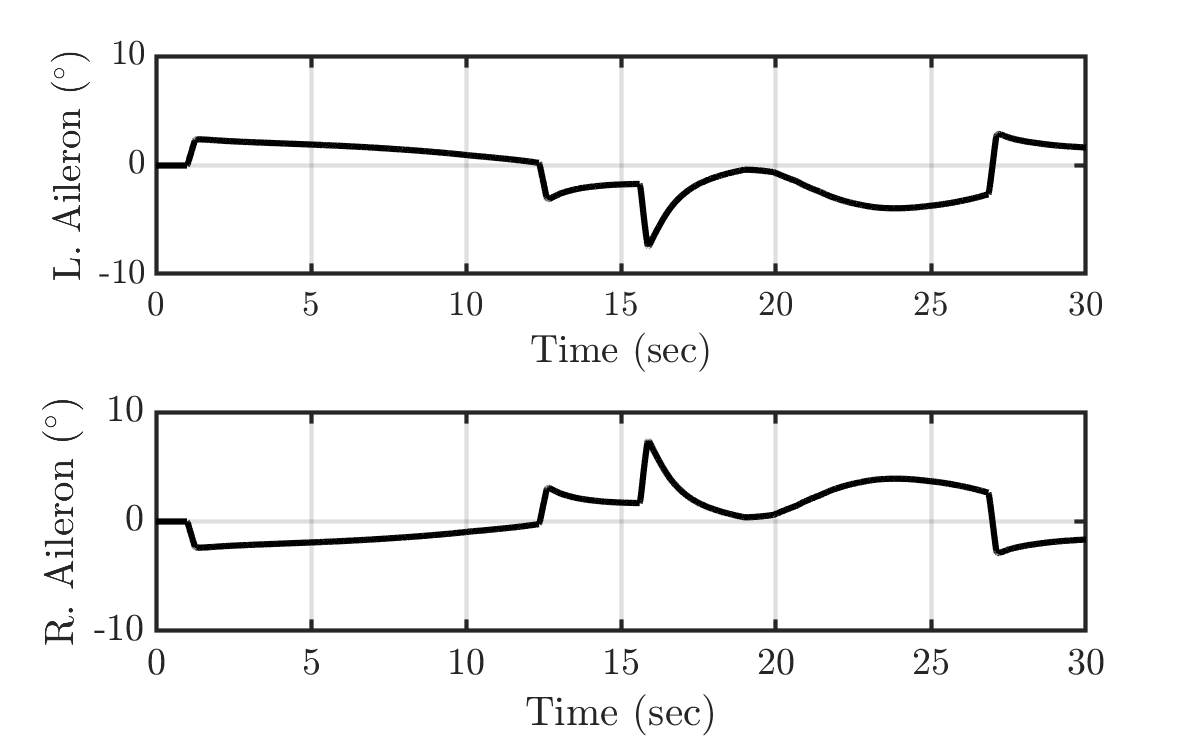
\includegraphics[trim=0 0 0 0, clip, width=.55\textwidth]{code/image_gen/cba/images/cfr147d_ail_defl.png} 
        \label{subfig:ail_defl}
    } 
    \end{subfigure}
    \caption{Steps required to convert the air-worthiness test into a the required inputs for the flight simulation of the maneuver. \label{fig:cfr147d_inputs}}
\end{figure}
 
\subsection{Monte Carlo Analysis}

\subsection{Modifications to the Simulation}